%% It is just an empty TeX file.
%% Write your code here.



%----------------------------------------------------------------------------------------
%	PACKAGES AND OTHER DOCUMENT CONFIGURATIONS
%----------------------------------------------------------------------------------------

\documentclass[12pt]{article} % Default font size is 12pt, it can be changed here

\usepackage{geometry} % Required to change the page size to A4
\geometry{a4paper} % Set the page size to be A4 as opposed to the default US Letter

\usepackage{graphicx} % Required for including pictures

\usepackage{float} % Allows putting an [H] in \begin{figure} to specify the exact location of the figure
\usepackage{wrapfig} % Allows in-line images such as the example fish picture


\linespread{1.2} % Line spacing

%\setlength\parindent{0pt} % Uncomment to remove all indentation from paragraphs

\graphicspath{{Pictures/}} % Specifies the directory where pictures are stored

\begin{document}

%----------------------------------------------------------------------------------------
%	TITLE PAGE
%----------------------------------------------------------------------------------------

\begin{titlepage}

\newcommand{\HRule}{\rule{\linewidth}{0.5mm}} % Defines a new command for the horizontal lines, change thickness here

\center % Center everything on the page

\textsc{\LARGE Enseeiht}\\[1.5cm] % Name of your university/college
\textsc{\Large Projet Long}\\[0.5cm] % Major heading such as course name
\textsc{\large Méthodes de clustering parallèles}\\[0.5cm] % Minor heading such as course title

\HRule \\[0.4cm]
{ \huge \bfseries Development Plan}\\[0.4cm] % Title of your document
\HRule \\[1.5cm]

\begin{minipage}{0.4\textwidth}
\begin{flushleft} \large
\emph{Project Manager:}\\
Tristan \textsc{Soriano} % Your name
\end{flushleft}
\end{minipage}
~
\begin{minipage}{0.4\textwidth}
\begin{flushright} \large
\emph{Supervisor:} \\
Laurent \textsc{Beugnet} % Supervisor's Name
\end{flushright}
\end{minipage}\\[4cm]

\begin{minipage}{0.4\textwidth}
\begin{flushleft} \large
\emph{Client IRIT:}\\
Ronan \textsc{Guivarch} % Your name
Sandrine \textsc{Mouysset}
\end{flushleft}
\end{minipage}




%{\large \today}\\[3cm] % Date, change the \today to a set date if you want to be precise

%\includegraphics{Logo}\\[1cm] % Include a department/university logo - this will require the graphicx package

\vfill % Fill the rest of the page with whitespace

\begin{figure}[H] % Example image
\center{
\includegraphics[width=0.5\linewidth]{Image/logo.jpg}}
\label{fig:speciation}
\end{figure}

\end{titlepage}

%----------------------------------------------------------------------------------------
%	TABLE OF CONTENTS
%----------------------------------------------------------------------------------------

\tableofcontents % Include a table of contents

\newpage % Begins the essay on a new page instead of on the same page as the table of contents 

%----------------------------------------------------------------------------------------
%	INTRODUCTION
%----------------------------------------------------------------------------------------

\section{Abstract} % Major section
It is a research project on image processing. It produces clustering creation among point sets and images.
A such treatment can be used for pattern recognition, image filtering or image segmentation.

\begin{figure}[h!] % Example image
\centering
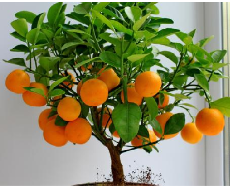
\includegraphics[width=0.5\linewidth]{Image/tree.png}

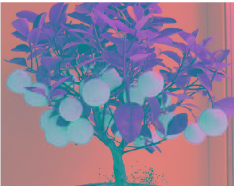
\includegraphics[width=0.5\linewidth]{Image/colortree.png}
\caption{ Example of clustering on the colors }

\end{figure}
%------------------------------------------------

\section{Presentation}

\subsection{Name} % Sub-section
New clustering methods integration into a parallel code.
\subsection{Sponsort}
IRIT : Ronan Guivarch, Sandrine Mouysset.
\subsection{Presentation}
The purpose of the project is to add new clustering methods into an existing piece of software. The clustering method are used on dense and sparse matrix which involve heavy computing calculus and time processing. In order to solve such issue, the existing code run on a master slave architecture. The original image is split among different slaves that compute initially a single clustering method : spectral clustering. 
\begin{figure}[H] % Example image
\center{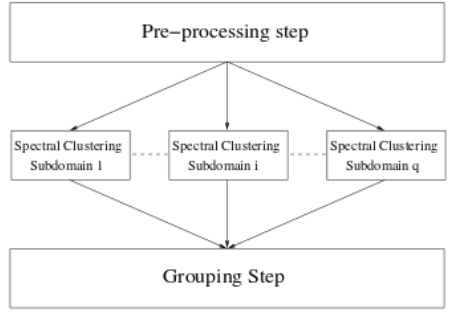
\includegraphics[width=0.5\linewidth]{Image/parallel.png}}
\caption{}
\label{fig:speciation}
\end{figure}
The objective is first to add two methods : Kernel K-means and Mean shift in such structure then to refactore/clean the existing code.


\section{Documentation}
The following reference can be used for any theoretical understanding of the algorithm. It also provides references on the minimum interface the different method must follow.

\begin{itemize}
\item The Global Kernel k-Means Clustering Algorithm
Grigorios Tzortzis and Aristidis Likas
\item The Variable Bandwidth Mean Shift and Data-Driven Scale Selection
Dorin Comaniciu
Visvanathan Ramesh 
Peter Meer
\item Mean Shift Analysis and Applications
Dorin Comaniciu
Peter Meer

\end{itemize}

\section{Domain}
\subsection{Included domain}
The project includes clustering method understanding, Fortran implementation, MPI.
\subsection{Excluded domain} 
We won't consider the parallel code optimization through libraries like OpenMP.

\section{Deliverable}
\begin{enumerate}
\item The team will produce spectral clustering, Kernel K-means and Mean Shift methods implemented in  Matlab with test validation : cible, croix, bouquet.
\item The team will provide configuration document for all the lab machine of Enseeiht : how to set up the environment, how to compile and run the program.
\item The team will produce new tests for spectral clustering  : 2D and 3D generated autogenerated tests.
\item It will be provided the existing Fortran code enhanced and cleaned :
	\begin{itemize}
	\item the quality of the code will be highlighted using a static analyzer
	\item the new modules Kernel K-means and mean shift
	\end{itemize}
\item Doxygen documentation will be provided : dependency graphs, method and parameters description.
\item The client will receive new tests for all the methods showing the interests of each method : advantages and drawbacks plus non regression tests comparing elapsed time and result quality.
\item The client will receive a PowerPoint presentation to explain the way the methods work.
\item The client will receive a test report with the test specification and result.
\end{enumerate}

\section{Communication}
\subsection{External communication}
The following schedule has been decided :
Weekly meeting with the client (IRIT) Sandrine Mouysset, Ronan Guivarch
\
Weekly meeting with the supervisor Laurent Beugnet
\
\subsection{Internal communication}
Biweekly meeting with the team to check the evolution of the project the possible issues and change of the planning depending on the progression
\
The text documentation can be found on Google Drive
\
The code and the examples can be found on  GitHub

\section{Development Management}
\subsection{Project organisation}
\subsubsection{Team}
The team is composed of five people :
\begin{itemize}
\item Project manager : Tristan Soriano is responsible for the communication between the team and the clients. He has to supervise the progress and the synchronization between the different parts
\item Quality manager : Simon Prieul ensures that the content produced by the team  reach the quality standards expected by the client.
\item Specification manager : Simon Aubeneau. He ensures that each piece of code produced match the specifications.
\item Validation manager : Quentin Duval is in charge of defining and running the tests.
\item Technical manager : Jéremy Santina manages the different technical and theoretical issues the team encounter.
\end{itemize}

\subsection{Work breakdown structure}
Each of the following step represents the schedule for the different point expected by the client to be complete. It check the good evolution of the project and the respect of the desired specifications.
\begin{description}
\item[Step 1]
	\begin{itemize}
	\item 1. Bibliography study (the reference can be found in the documentation section)
 	\item 2. Existing parallel code set up on lab machines , new example creation : 2D examples 3D exemples
	\item 3. The three following methods must be implemented in matlab : spectral clustering, Kernel K­means et Mean Shift        
	\end{itemize} 
\item[Step 2]
	\begin{itemize}
	\item 1. Code documentation (Doxygen) : dependency graphs, method and parameters description.
	\item 2. End of the clustering methods implementation in Matlab
	\end{itemize}
\item[Step 3]
	\begin{itemize}
	\item This step provides specification of the new clustering methods interfaces FORTRAN and validation with the client.
	\end{itemize}
\item[Step 4]
	\begin{itemize}
	\item 1. Code refactoring : the code will follow classical FORTRAN coding convention, the method and variables will be renamed for better understanding.
	\item 2. Implementation of the new clustering methods interfaces FORTRAN
	\item 3. new tests generation
	\end{itemize}
\item[Step 5]
	\begin{itemize}
	\item Validation of the new methods. Quality of the result on the different tests, time elapsed computing, non regression check.
	\item The refactored code will be tested and the validation will rely on statical analysis of the code
	\end{itemize}
\end{description}




\section{Risk management}
\begin{figure}[htb]

\begin{center}
\begin{tabular}{|p{5cm}|p{3cm}|p{2cm}|p{5cm}|} 
\hline \textbf{Description} &  \textbf{Probability} &  \textbf{Impact} & \textbf{Action} \\
\hline  The product do not fit the client expectation. &  light & heavy &  specification with the client \\
\hline Resources inadequate & medium & heavy & lighter test creation, request access on computers \\
\hline Insufficient knowledge & Heavy & Medium & increase the time dedicated to each risky task \\
\hline
\end{tabular}
\end{center}
\end{figure}


\section{Gantt} 
\begin{tabular}{|c|c|c|c|c|}
\hline \textbf{Member} & \textbf{Action} & \textbf{Begin} & \textbf{End} \\ 
\hline Tristan Soriano  & Etude théorique & 01/18/15 & 02/04/15  \\ 
\hline Simon Prieul & Installation \& wikiHow & 01/18/15 & 01/30/15 \\
\hline Simon Aubeneau  & Installation \& wikiHow & 01/18/15 & 01/30/15 \\
\hline Quentin Duval  & Etude théorique & 01/18/15 & 02/04/15 \\
\hline Jéremy Santina  & & & \\

\hline Tristan Soriano & Implementation Matlab & 02/02/15 & 02/11/15 \\
\hline Quentin Duval & Implementation Matlab & 02/02/15 & 02/11/15 \\
\hline Jéremy Santina & Etude du code existant \& Doc Doxygen & 02/02/15 & 02/11/15 \\
\hline Simon Aubeneau & Etude du code existant \& Doc Doxygen & 02/02/15 & 02/11/15 \\
\hline Simon Prieul & Etude du code existant \& Doc Doxygen & 02/02/15 & 02/11/15 \\
\hline Tristan Soriano & Interface des nouvelles méthodes & 02/15/15 & 02/22/15 \\
\hline Quentin Duval & Refactoring du code & 02/15/15 & 02/25/15 \\
\hline Jéremy Santina & Interface des nouvelles méthodes & 02/15/15 & 02/22/15 \\
\hline Simon Aubeneau & Refactoring du code & 02/15/15 & 02/25/15 \\
\hline Simon Prieul & Interface des nouvelles méthodes & 02/15/15 & 02/22/15 \\
\hline Tristan Soriano & Implémentation des nouvelles méthodes & 02/22/15 & 03/08/15 \\
\hline Quentin Duval & Implémentation des nouvelles méthodes & 02/22/15 & 03/08/15 \\
\hline Jéremy Santina & Implémentation des nouvelles méthodes & 02/22/15 & 03/08/15\\
\hline Simon Aubeneau & Refactoring du code & 02/22/15 & 03/08/15 \\
\hline Simon Prieul & Refactoring du code & 02/22/15 & 03/08/15 \\
\hline Tristan Soriano & Validation & 03/08/15 & 03/12/15 \\
\hline Quentin Duval & Validation & 03/08/15 & 03/12/15 \\
\hline Jéremy Santina & Validation & 03/08/15 & 03/12/15 \\
\hline Simon Aubeneau & Validation & 03/08/15 & 03/12/15 \\
\hline Simon Prieul & Validation & 03/08/15 & 03/12/15 \\
\hline 
 
\end{tabular}  

\begin{figure}[H] % Example image
\center{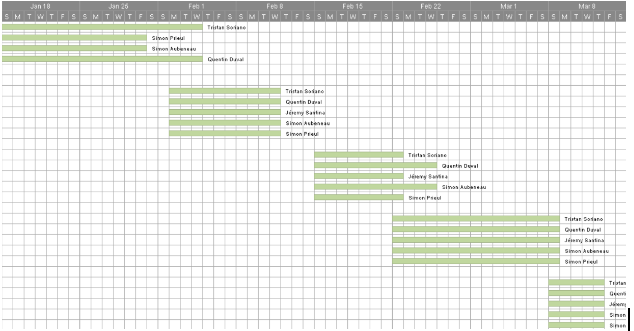
\includegraphics[width=1\linewidth]{Image/gantt1111.png}}
\label{fig:specification}
\end{figure}


\end{document}